\documentclass{beamer}
\usetheme{Copenhagen}
\usepackage{tikz}
\usepackage{multirow}
\usepackage{graphicx}
\usepackage{epstopdf}
\usepackage{subfigure}
\graphicspath{{img/}}

\title[Nomadic Computing for Big Data Analytics]{Nomadic Computing for Big Data Analytics}
\institute{}
\author[Delivered by Chen Shaoyuan]{Original authors: Hsiang-Fu Yu, Cho-Jui Hsieh, Hyokun Yun, S.V.N. Vishwanathan, Inderjit Dhillon}
\date{November 15, 2017}

\renewcommand{\vec}{\mathbf}
\setlength{\parskip}{0.2cm}

\begin{document}
  \begin{frame}
    \titlepage
  \end{frame}

  \section{Introduction}
  \begin{frame}{Introduction}{Analysis of big data}
    Two approaches of big data analysis
    \begin{itemize}
      \item Stochastic optimization \& inference (sequential);
      \item Distributed computing based on MapReduce.
    \end{itemize}
    \pause
    Stochastic optimization and inference algorithms are inherently sequential, making them hard to be run on distributed system. \par
    \pause
    NOMAD (Nonlocking, stOchastic Multimachine framework for Asynchronous and Decentralized computation), is presented in this paper, which combines stochastic optimization's and distributed computing's advantages without incurring their drawbacks.
  \end{frame}
  
  \section{Matrix Completion}
  \begin{frame}{Matrix Completion}{Some notations}
    \begin{tabbing}
      Notation $\quad$ \=  Meaning \\
      % \> for next tab, \\ for new line...
      $\langle \cdot , \cdot \rangle$ \> the Euclidean inner product of two vectors \\
      $\Omega_i$ \> $\{j : (i, j) \in \Omega\}$ \\
      $\overline{\Omega}_j$ \> $\{i : (i, j) \in \Omega\}$ \\
      $|\cdot|$ \> The cardinality of a set \\
      $\| \cdot \|$ \> The $L^2$ norm of a vector \\
      $[a..b]$ \> $\{a, a+1, \cdots, b\}$
    \end{tabbing}
  \end{frame}
  
  \begin{frame}{Matrix Completion}{The problem}
    \begin{block}{Matrix completion problem}
    Given an incomplete matrix $A \in R^{m \times n}$, where only entries of indices $(i, j) \in \Omega \subset [1 .. m] \times [1 .. n]$ are known. The task is to find two matrices $W \in R^{m \times k}$ and $H \in R^{k \times  n}$ with $k \ll \min\{m,n\}$, such that $A \approx WH^{\text{T}}$.
    \end{block}
    \pause
    The matrix $W$ can be considered as $m$ $k$-dimensional row vectors, and $H$ as $n$ $k$-dimensional column vectors. Then, for every entry $A_{ij}$, it is simply the inner product of the corresponding row and column vectors:
  $$ A_{ij} = \langle \vec{w}_i, \vec{h}_j \rangle$$ 
  \end{frame}
  
  \begin{frame}{Matrix Completion}{The problem}
    We use loss function to measure the goodness of the model, typically given by mean squared error: 
    $$ \frac{1}{2|\Omega|} \sum_{(i, j) \in \Omega} (A_{ij} - \langle \vec{w}_i, \vec{h}_j \rangle)^2 $$
    also, we need a regularizer to avoid overfitting
    $$ \frac{\lambda}{2} ( \sum_{i = 1}^m | \Omega_i | \cdot \|\vec{w}_i\|^2 + \sum_{i=1}^n | \overline{\Omega}_j| \cdot \|\vec{h}_j\|^2) $$
    Combine these two items, the problem can be described as
    $$\min_{W, H} J(W, H) = \frac{1}{2|\Omega|} \sum_{(i, j) \in \Omega} (A_{ij} - \langle \vec{w}_i, \vec{h}_j \rangle)^2 + \text{regularizer}$$
  \end{frame}
  
  \begin{frame}{Matrix Completion}{Stochastic gradient descent}
    Take the gradients of the target function with respect to $\vec{w}_i$ and $\vec{h}_j$:
    \begin{align*}
      \nabla_{\vec{w}_i}J(W, H) &= -(A_{ij} - \langle \vec{w}_i, \vec{h}_j \rangle) \vec{h}_j + \lambda \vec{w}_i \\
      \nabla_{\vec{h}_j}J(W, H) &= -(A_{ij} - \langle \vec{w}_i, \vec{h}_j \rangle) \vec{w}_i + \lambda \vec{h}_j 
    \end{align*}
    \pause
    The function decrease at the greatest rate in the opposite direction of the gradient of a function points, so we tend to move our approximation to somewhere in the opposite the direction of the gradient:
    \begin{align}
      \vec{w}_i &\leftarrow \vec{w}_i - s_t [-(A_{ij} - \langle \vec{w}_i, \vec{h}_j \rangle) \vec{h}_j + \lambda \vec{w}_i] \\
      \vec{h}_j &\leftarrow \vec{h}_j - s_t [-(A_{ij} - \langle \vec{w}_i, \vec{h}_j \rangle) \vec{w}_i + \lambda \vec{h}_j]
    \end{align}
    where $s_t$ is called the learning rate.
  \end{frame}
  
  \begin{frame}{Matrix Completion}{Stochastic gradient descent}
    Repeatedly performing such updates, we will finally obtain an optimal result within admissible error. However, computing all the gradients and updating all the vectors take too much time. \par
    The main idea of stochastic gradient descent, is that we randomly choose a pair of vectors $\vec{w}_i, \vec{h}_j$, calculate the gradients with respect to the two vectors, and perform updates (1) and (2).
  \end{frame}
  
  \begin{frame}{Matrix Completion}{NOMAD in matrix completion}
    Note that, to update $\vec{w}_i$ and $\vec{h}_j$, one only need to know $\vec{w}_i$, $\vec{h}_j$ and $A_{ij}$. To parallelize the process, we partition the indices $[1..m]$ to $p$ disjoint sets $I_1, I_2, \cdots, I_p$ of approximately equal size, each worker processes one set. The data is partitioned and distributed in the following ways:
    \pause
    \begin{itemize}
      \item The $q$-th worker stores $\overline{\Omega}^{(q)}_j := \{(i, j) \in \overline{\Omega}_j; i \in I_q\}$;
      \item The $q$-th worker stores $\vec{w}_i, i \in I_q$ and $A_{ij}, i \in I_q$;
      \item The vectors $\vec{h}_j$ are randomly distributed to the workers at the beginning, and moving between the workers during processing.
    \end{itemize}
  \end{frame}
  
  \begin{frame}{Matrix Completion}{NOMAD in matrix completion}
    Note that, to update $\vec{w}_i$ and $\vec{h}_j$, one only need to know $\vec{w}_i$, $\vec{h}_j$ and $A_{ij}$. To parallelize the process, we partition the indices $[1..m]$ to $p$ disjoint sets $I_1, I_2, \cdots, I_p$ of approximately equal size, each worker processes one set. The data is partitioned and distributed in the following ways:
    \pause
    \begin{itemize}
      \item The $q$-th worker stores $\overline{\Omega}^{(q)}_j := \{(i, j) \in \overline{\Omega}_j; i \in I_q\}$;
      \item The $q$-th worker stores $\vec{w}_i, i \in I_q$ and $A_{ij}, i \in I_q$;
      \item The vectors $\vec{h}_j$ are randomly distributed to the workers at the beginning, and moving between the workers during processing.
    \end{itemize}
  \end{frame}
  
  \begin{frame}{Matrix Completion}{NOMAD in matrix completion}
    \begin{figure}
      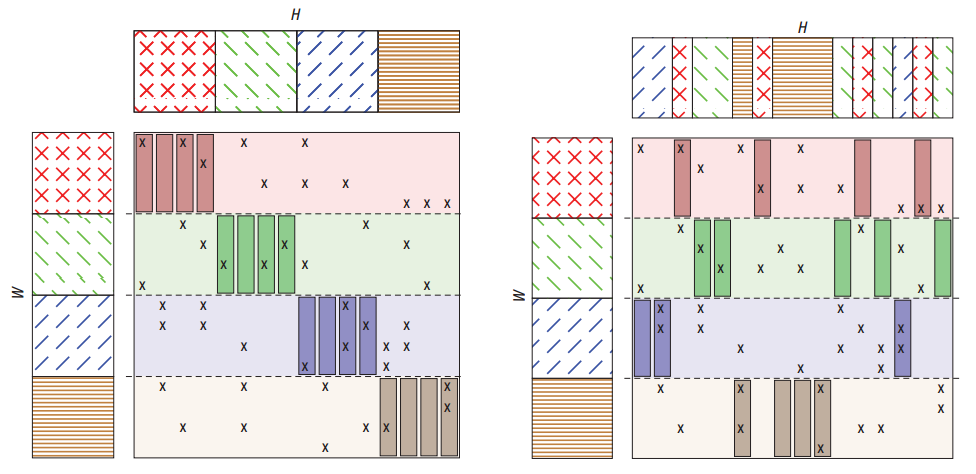
\includegraphics[height = 5cm]{mc_data.png}
      \caption{Ownership of the data}
    \end{figure}
  \end{frame}
  
  \begin{frame}{Matrix Completion}{NOMAD in matrix completion}
    Every worker randomly chooses an index $i \in I_q$ and vector $\vec{h}_j$ it owns, and update vectors $\vec{w}_i$ and $\vec{h}_j$. The worker transfers the ownership of vector $\vec{h}_j$ to another worker immediately after the update. \par
    \pause
    The advantages of this scheme are
    \begin{itemize}
      \item Decentralized;
      \item Asynchronous computation and communication;
      \item Serializability.
    \end{itemize}
    \pause
    Disadvantages?
  \end{frame}
  
  \begin{frame}{Matrix Completion}{NOMAD in matrix completion}
    \begin{figure}
      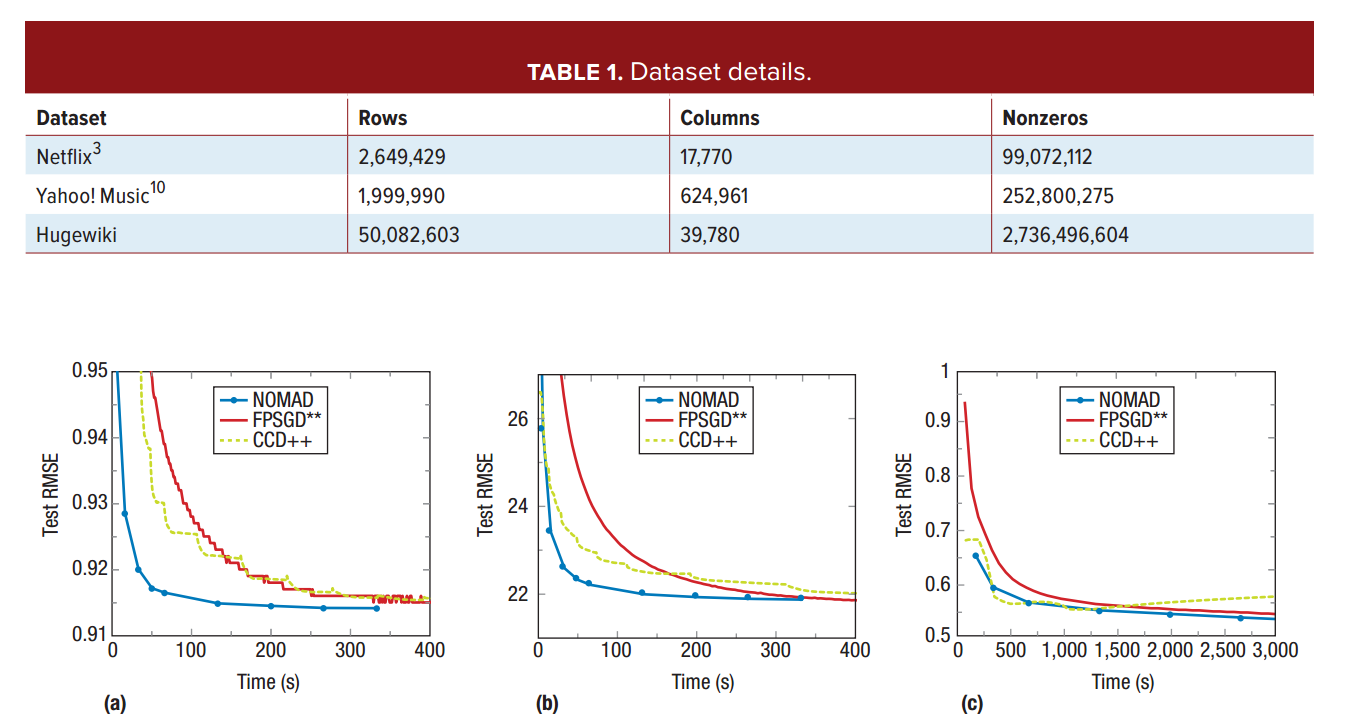
\includegraphics[height = 5cm]{mc_perform.png}
      \caption{Performance of NOMAD in matrix completion}
    \end{figure}
  \end{frame}

  
  \section{Latent Dirichlet Allocation}
  \begin{frame}{Latent Dirichlet Allocation}{Some notations}
    Suppose we are given $I$ documents.
    \begin{tabbing}
      Notation $\quad$ \=  Meaning \\
      % \> for next tab, \\ for new line...
      $d_i$ \> the $i$th document \\
      $n_i$ \> number of words in the $i$th document \\
      $w_{i, j}$ \> the $j$th word in the $i$th document \\
      $z_{i, j}$ \> the latent topic from which $w_{i, j}$ was drawn \\
      $n(z, i, w)$ \> $\sum_{j = 1}^{n_i} I(z_{i, j} = z \wedge w_{i, j} = w) $ \\
      $n(z, i, *)$ \> $\sum_{w} n(z, i, w)$ \\
      $n(z, *, w)$ \> $\sum_{i} n(z, i, w)$ \\
      $n(z, *, *)$ \> $\sum_{i, w} n(z, i, w)$ 
    \end{tabbing}
  \end{frame}
  
  \begin{frame}{Latent Dirichlet Allocation}{Some notations}
    \begin{tabbing}
      Notation $\quad$ \=  Meaning \\
      % \> for next tab, \\ for new line...
      $\vec{n}_t$ \> the vector $n(z, *, *)$ over $z$ \\
      $\vec{n}_w$ \> the vector $n(z, *, w)$ over $z$ \\
      $\vec{n}_d$ \> the vector $n(z, d, *)$ over $z$ 
    \end{tabbing}
  \end{frame}
  
  \begin{frame}{Latent Dirichlet Allocation}{Collapsed Gibbs sampling}
    The inference task for LDA requires Collapsed Gibbs sampling (CGS). \par
    \pause
    The update rule for CGS of indices $(i, j)$ can be written as 
    \begin{enumerate}
      \item Decrease $n(z_{i, j}, i, *)$, $n(z_{i, j}, *, w_{i, j})$ and $n(z_{i, j}, *, w_{i, j})$ by 1;
      \item Resample $z_{i,j}$ according to:
      $$ \text{Pr}(z_{i, j} | w_{i, j}, \alpha, \beta) \propto \frac{(n(z_{i,j},i,*)+\alpha)(n(z_{i,j},*,w_{i,j})+\beta)}{n(z_{i,j}, *, *) + J \cdot \beta} $$
      \item Increase $n(z_{i, j}, i, *)$, $n(z_{i, j}, *, w_{i, j})$ and $n(z_{i, j}, *, w_{i, j})$ by 1.
    \end{enumerate}
  \end{frame}
  
  \begin{frame}{Latent Dirichlet Allocation}{Nomadic approach for LDA}
    To perform an update, we need to access $z_{i, j}, \vec{n}_w, \vec{n}_d$ and $\vec{n}_t$. If there is no $\vec{n}_t$, the access pattern is identical to that of matrix completion problem. \par
    \pause
    Note that, the elements in $\vec{n}_t$ are very large, and any small change to $\vec{n}_t$ is negligible. This enables us to design a special nomadic scheme for $\vec{n}_t$:
    \begin{itemize}
      \item There is only one worker keeps $\vec{n}_t$, while each worker has its own local copy $\vec{n}_t^{(i)}$;
      \item Whenever a worker receives $\vec{n}_t$, it updates $\vec{n}_t$ with the change in its local copy, keeps a snapshot $\vec{\bar{n}}_t$, and passes $\vec{n}_t$ to the next worker.
    \end{itemize}
  \end{frame}
  
  \begin{frame}{Latent Dirichlet Allocation}{Nomadic approach for LDA}
    \begin{figure}
      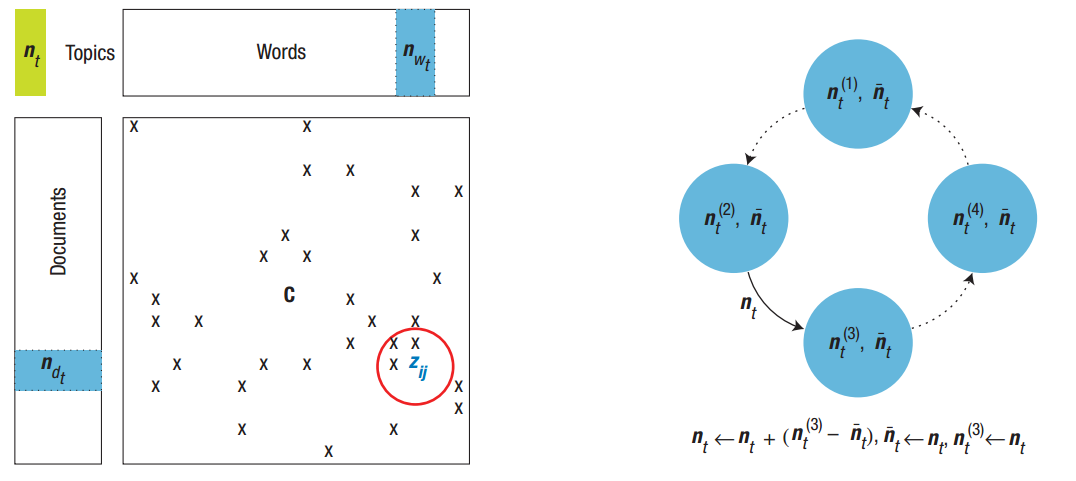
\includegraphics[height = 5cm]{cgs_data.png}
      \caption{Data access graph and the nomadic scheme for $\vec{n}_t$}
    \end{figure}
  \end{frame}
  
  \begin{frame}{Latent Dirichlet Allocation}{Nomadic approach for LDA}
    \begin{figure}
      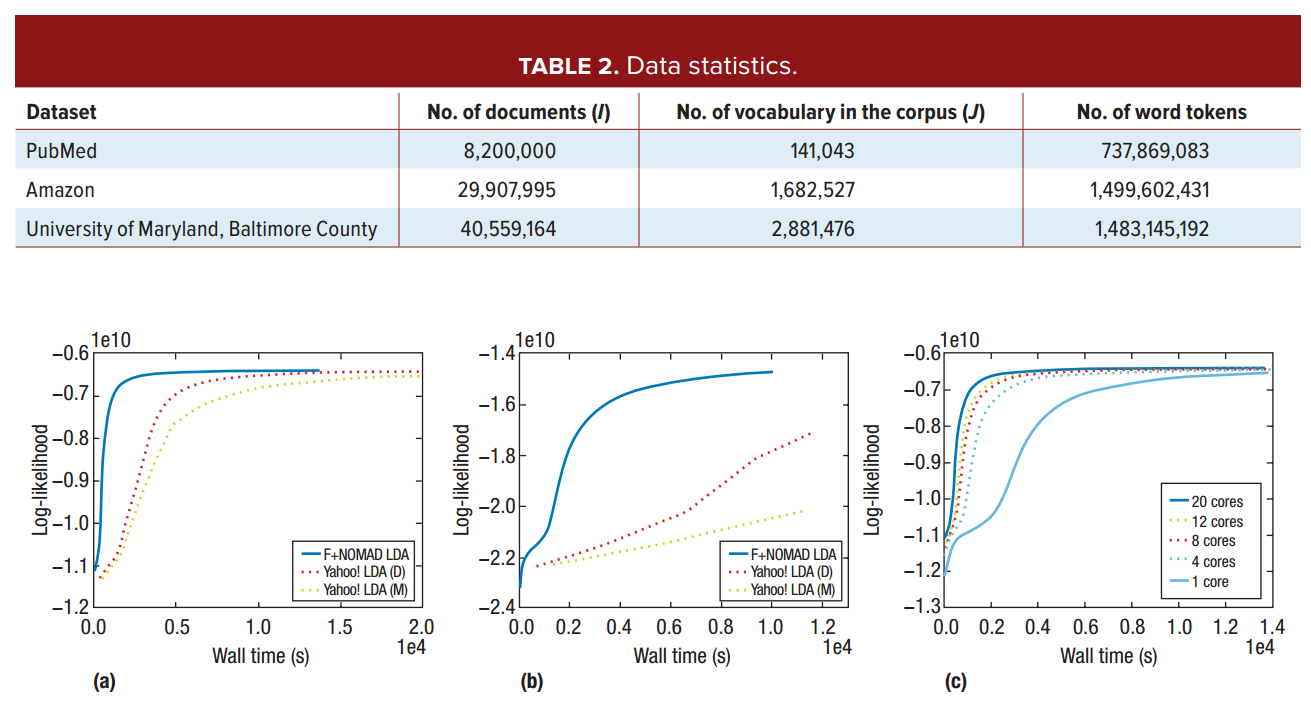
\includegraphics[height = 5.5cm]{cgs_perform.png}
      \caption{Performance of NOMAD for LDA}
    \end{figure}
  \end{frame}
  
  \section{Summary}
  
  \section{}
  \begin{frame}{Q \& A}

  \end{frame}
\end{document}
